\documentclass[11pt]{article}
\usepackage{graphicx}
\usepackage[utf8]{inputenc}
\usepackage{amsmath}
\usepackage{gensymb}
\usepackage{setspace}
\usepackage{caption}
\usepackage{subcaption}
\usepackage{wrapfig}
\usepackage{caption}
\captionsetup[figure]{font=footnotesize}
\usepackage{csvsimple}
\usepackage{lineno}
\usepackage{amssymb}
\usepackage{amsmath}
\usepackage{harvard}
\usepackage{parskip}
\usepackage[a4paper,width=150mm,top=20mm,bottom=20mm,bindingoffset=6mm]{geometry}
\usepackage{fancyhdr}
\pagestyle{fancy}
\fancyhead{}
\fancyhead[CE]{Model Selection in Microbial Population Growth}

\doublespacing

\begin{document}

\begin{titlepage}
    \begin{center}
    \vspace*{1cm}

    \Huge
    \textbf{\underline{Modelling the effects of Gene Flow and Selection on the Canalisation}}\\
    \textbf{\underline{of an established Genetic Network}}\\

    \vspace*{2.0cm}

    \large
    \textbf{Author: Matthew Campos}\\
    \textbf{Submitted August 2020}

    \vspace*{0.8cm}

    \normalsize
    A thesis submitted in partial fulfilment of the requirements for the degree of Master of Science/Research at Imperial College London\\
    Formatted in the journal style of Evolution \& Development\\
    Submitted for the MSc in Computational Methods in Ecology and Evolution\\

    \vspace*{0.8cm}

    \end{center}
\end{titlepage}


\newpage

\linenumbers

\section*{Abstract}
The purpose of this research is to identify appropriate models that can give insight into microbial population data. Model derivations and fitting have become a popular approach to hypothesis testing, being able to describe and explain trends and patterns in data. Using published data and different software packages and functions, the data was manipulated and fit with chosen population ecology models. The Akaike Information Criterion was the statistical method chosen to identify which models fit the data best. Four mechanistic models were chosen and the Gompertz model performed best for the given data set. Its derivations and parameters allow it to be a robust and flexible model. An additional study was conducted to see the correlation between growth rate and temperature. The findings show that they are positively correlated and almost follow a linear pattern.

\newpage

\section*{Acknowledgements}
I would like to thank Dr.Pawar and Dr.Rosindell for leading the master's course, providing support and guidance throughout. To Dr.Pawar's laboratory team for providing us with the data, to Ph.D Tom Clegg and Ph.D Katie Willis for having Monday help sessions for this Miniproject.

\newpage

\tableofcontents

\newpage

\section{Introduction}
Mathematical models can be used to explain or describe natural phenomena and observations. This method of modelling can be applied in the field of Ecology and Evolution. Models fitting is a simplistic method to describe the general behaviour of long-term macro-biological events noticed in nature \cite{johnson2004model}. Generalised models can be applied in population ecology and can explain different observed phenomena including the dynamics of population growth, and how factors and conditions affect these populations over time. The models chosen are generalised models describing bacterial growth. Therefore, they disregard the capacity for evolution, classifying the organisms as homogenous \cite{levins1966strategy}. Finding the best fit will be achieved by fitting suitable models and evaluating them using either maximum likelihood or least squares \cite{johnson2004model}. If carried out properly, parameters and overall function of the model are used to make biological inferences on the patterns recorded \cite{johnson2004model}. The challenge, however, is finding the appropriate model and taking into considerations the assumptions and trade-offs of these different models.

Models aim explain the important aspects of the data, thus have many assumptions. When choosing a model, it is important to account for the trade-offs between generality, realism and precision. In other words, the purpose of the model, and what is being investigated is an important factor. Models should focus on sustaining generality and realism, as they are able to quantitatively explain long-term trends that the data reveals \cite{levins1966strategy}.  In addition to this, ensuring that the parameters have biological significance rather than just statistical significance \cite{johnson2004model}. For this project, identifying the correct model is achieved through the process of testing multiple existing models on the data and identifying the best fits on the data using the analytical method of Maximum Likelihood. The outcome should be plausible models that for observed data, consistently describes the patterns in these observations mechanistically or empirically.

The focus of this project is to test multiple non-linear regression models on microbial population data. Identifying the best models that best fit and or describe the pattern of the data provided. Microbes grow through a process known as binary fission, doubling the population continually \cite{webb1986logistic}. This exponential growth coupled with limiting factors gives microbial population growth a sigmoidal shape which can be divided into four phases \cite{peleg2011microbial}. The trend begins with birth, a starting population ($N_0$) and growth where limiting factors is not yet inhibiting, thus having an exponential growth curve, with a growth rate notation of $r_{max}$ \cite{zwietering1990modeling}. Limiting factors such as space, nutrients and particularly carrying capacity can inhibit growth, resulting in the rate of growth to decrease and eventually reaches saturation, becoming asymptotic. The asymptotic value being the carrying capacity, with the notation $N_{max}$ \cite{zwietering1990modeling}.

Four mechanistic models will be tested on the data set. These are the Logistic Growth Model \cite{bacaer2011verhulst}, Baranyi Model (Baranyi,1993), Gompertz Model \cite{zwietering1990modeling} and Buchanan Model \cite{buchanan1997simple}, 1997), given below.

\textit{Logistic Model}
\begin{equation*}
    N_t = \frac{N_0 \cdot N_{max} \cdot e^{r_{max} \cdot t}}{N_{max} + N_0(e^{r_{max} \cdot t} -1)} \label{eq:Logistic Model} \tag{1.1}
\end{equation*}

\textit{Baryani Model}
\begin{equation*}
    N_t = N_{max} + \log_{10}(\frac{-1 + \exp(r_{max} \cdot t_{lag}) + \exp(r_{max} \cdot t)}{\exp(r_{max} \cdot t) - 1 + \exp(r_{max} \cdot t_{lag}) \cdot 10^(N_{max} - N_0)}) \label{eq:Baranyi Model} \tag{1.2}
\end{equation*}

\textit{Gompertz Model}
\begin{equation*}
    N_t =  N_0 + (N_{max} - N_0) \cdot \frac{\exp(-\exp(r_{max} \cdot \exp(1) \cdot (t_{lag} - t)}{(N_{max} - N_0) \cdot \ln(10) + 1})) \label{eq:Gompertz Model} \tag{1.3}
\end{equation*}

\textit{Buchanan Model}
\begin{equation*}
    N_t = \begin{cases}
          N_0, & \text{if } t\leq t_{lag}\\
          N_{max} + r_{max} \cdot (t - t_{lag}), & \text{if } t_{lag} < t < t_{max}\\
          N_{max}, & \text{if } t\geq t_{max}
          \end{cases} \label{eq:Buchanan Model} \tag{1.4}
\end{equation*}
Model fits be will be assessed using the Akaike Information Criterion (AIC), which is a relative comparison where the best fit is the model with the minimum value \cite{vrieze2012model, posada2004model}. The AIC is a criterion used to assess the model fits. It is a relative measure of the Kullback-Leibler divergence estimate. Meaning that whereas the K-L divergence measures the deviation of a model from the "true model", the AIC is an estimate value only between the models considered \cite{vrieze2012model}. It consists of two variables, the likelihood function (a loss function) which results in a Maximum Likelihood Estimate of the parameters, and the number of parameters in the model \cite{vrieze2012model}. The formual is given below, where $\alpha$ is known as the penalty coefficient (with a value of 2), $\kappa$ is the number of parameters and $\mathcal{L}$ is the Maximum Likelihood Estimate of the parameters.

\textit{Akaike Information Criterion}
\begin{equation*}
    AIC = -2 \cdot \ln{(\mathcal{L})} + \alpha \cdot \kappa \label{eq:AIC} \tag{2}
\end{equation*}
Lastly, an additional investigation on the correlation between growth rate and temperature is also carried out. In addition to this, compare two models, a linear model and a relationship formula given by \textit{Ratkowsky et al.} Given the range of temperature from 0 degrees Celsius to 37 degrees Celsius, the expectation is to see a positive linear relationship between increasing temperature and growth rate. Species and medium are factors considered and a linear regression anlaysis is carried out for correlation. The linear slope is also tested adjacent to a formula from \textit{Ratkowsky et al.} given below.

\begin{equation*}
    \sqrt{r}=b(T-T_0) \label{eq:Conceptual Temperature model} \tag{3}
\end{equation*}
I will call this formula the Conceptual Temperature model. The parameter $T_0$ is the conceptual temperature, a hypothetical temperature which has no metabolic significance, in which other factors such as medium are non-limiting \cite{ratkowsky1982relationship} Conceptual temperatures for different species are provided from \textit{Ratkowsky et al.} paper and used to identify the relationship between growth rate and temperature.

\section{Methods}
In this project, published data was provided from multiple experiments on microbial population and growth. Growth conditions including medium and temperature were manipulated and populations were recorded through different measurements techniques. The Population numbers and time were recorded discretely at different time intervals. The data were stored in a \textit{.csv} file, manipulated and fitted with the models through different software packages.\\

\subsection{Computing Tools}
\textit{Python}

Python 3.7.1 software was used to explore the data. The data provided was in one large \textit{.csv} file and needed to be manipulated before being filtered. Combination of functions and commands were used to wrangle the data and remove unwanted data points, as well as converting to log space. \textit{Pandas} and \textit{Numpy} were the two packages used for the purpose of data import and carrying out mathematical manipulations of the data set.

\textit{R}

R 3.6.1 software was used to filter the data set and carry out data analysis. Software package \textit{dplyr} was used to filter the data set and create unique ID’s, which were saved as \textit{.rda} files. The mechanistic equations to be fitted on the data and functions to find optimal starting value for the parameters were done in R. Using \textit{minpack.lm} package, non-linear regression analysis was carried out using the \textit{nlsLM()} function as well as plotting the different unique analysis. The package BisRNA was used to perform fisher's method to get a p-value statistic from multiple independent tests for the linear regression of growth rate and temperature. The \textit{stringr} package was used for setting wrappers and filtering the unique species by their string. Lastly, \textit{gridExtra} package was used to save tables from R in pdf format.

\textit{Bash}

Bash script was used to run the python, R scripts and the latex file, to convert the latex into a pdf.

\subsection{Data Exploration and Filtering}

The data was first wrangled before being filtered. All abundance recordings of OD595 were first multiplied by 100. Next the data was treated in linear scale, therefore negative time and population values were either removed or shifted, with negative time values set to zero. The data was then transformed to a log scale, by taking the common logarithm of the population abundance. This is to fit the criteria of three of the models and make the data less skewed. Although the Logistic model is not in log scale, the output value is of the function is, to maintain the linearity of the function.

Data was then filtered based on the headings: species, medium, temperature, citation and replicate. It is important to note that method of collecting population count was not a factor in the model fitting and assessing of best model(s). The unique data sets were saved in .rda files which included the unique ID’s and a data frame of the time intervals, labelled Time and the common logarithm of the population count at each discrete time interval, labelled Abundance.

The four mechanistic models were then fitted to all the different sub-data sets. Of the four, the Logistic formula is derived from bacterial growth properties, where $r_{max}$ is the maximum growth rate in the exponential phase and $N_{max}$ represents the carrying capacity. Since all the models utilise the same parameters, their values can be interpreted to have the same biological interpretations (Levins 1996). Using R Programming Language, each of the models will be tested on the data and the Akaike Information Criterion (AIC) will be the statistic to analyse the model of best fit.

\subsection{Estimating parameters values for Model Fitting}

$N_0$ is the starting population value at the first-time recording, thus the first data point. The carrying capacity ($N_{max}$) is the largest value found in the data set, which is the maximum value of the data set. The growth rate, $r_{max}$, is the largest gradient value of the derivative found at the point $\frac{N_{max}}{2}$, otherwise known as the inflection point. To find the estimate of this parameter, a function utilising a while loop was used. It describes the rate of change of the population over time, given the equation below:
\begin{equation*}
    \frac{dx}{dt}=\frac{x_{i+1}-x_{i}}{t_{i+1}-t_{i}}\label{eq:slope} \tag{4}
\end{equation*}
Where $dx$ represents the change in population count from time $i$, to time, $i+1$. Starting from the first data point and iterating to the final two data points, each iteration calculated the slope between the adjacent data points, saving all results in a vector and the largest value was taken to be the $r_{max}$. Any negative growth rate slopes $r_{max}$ would be set to NA, to prevent model fitting

The models include a time lag, which is a delay in time of bacteria growth. The estimation is found through the intersection between the lag phase, which can be represented by the starting population value, and exponential growth phase, represented by the slope of the growth rate \cite{peleg2011microbial}. This was calculated by the intersection of y=$N_0$ and the line with gradient $r_{max}$. Using the y-intercept ($y_{int}$) value from the $r_{max}$ line. Rearranging of the linear equation leads to the formula:
\begin{equation*}
   t_{lag}=\frac{N_0 - y_{int}}{r_{max}}
\end{equation*}
Should $t_{lag}$ be negative, but the $r_{max}$ positive, its value would be set to $0$. Figure 1 below shows an example of this derivation.
\begin{figure}[h]
\centering
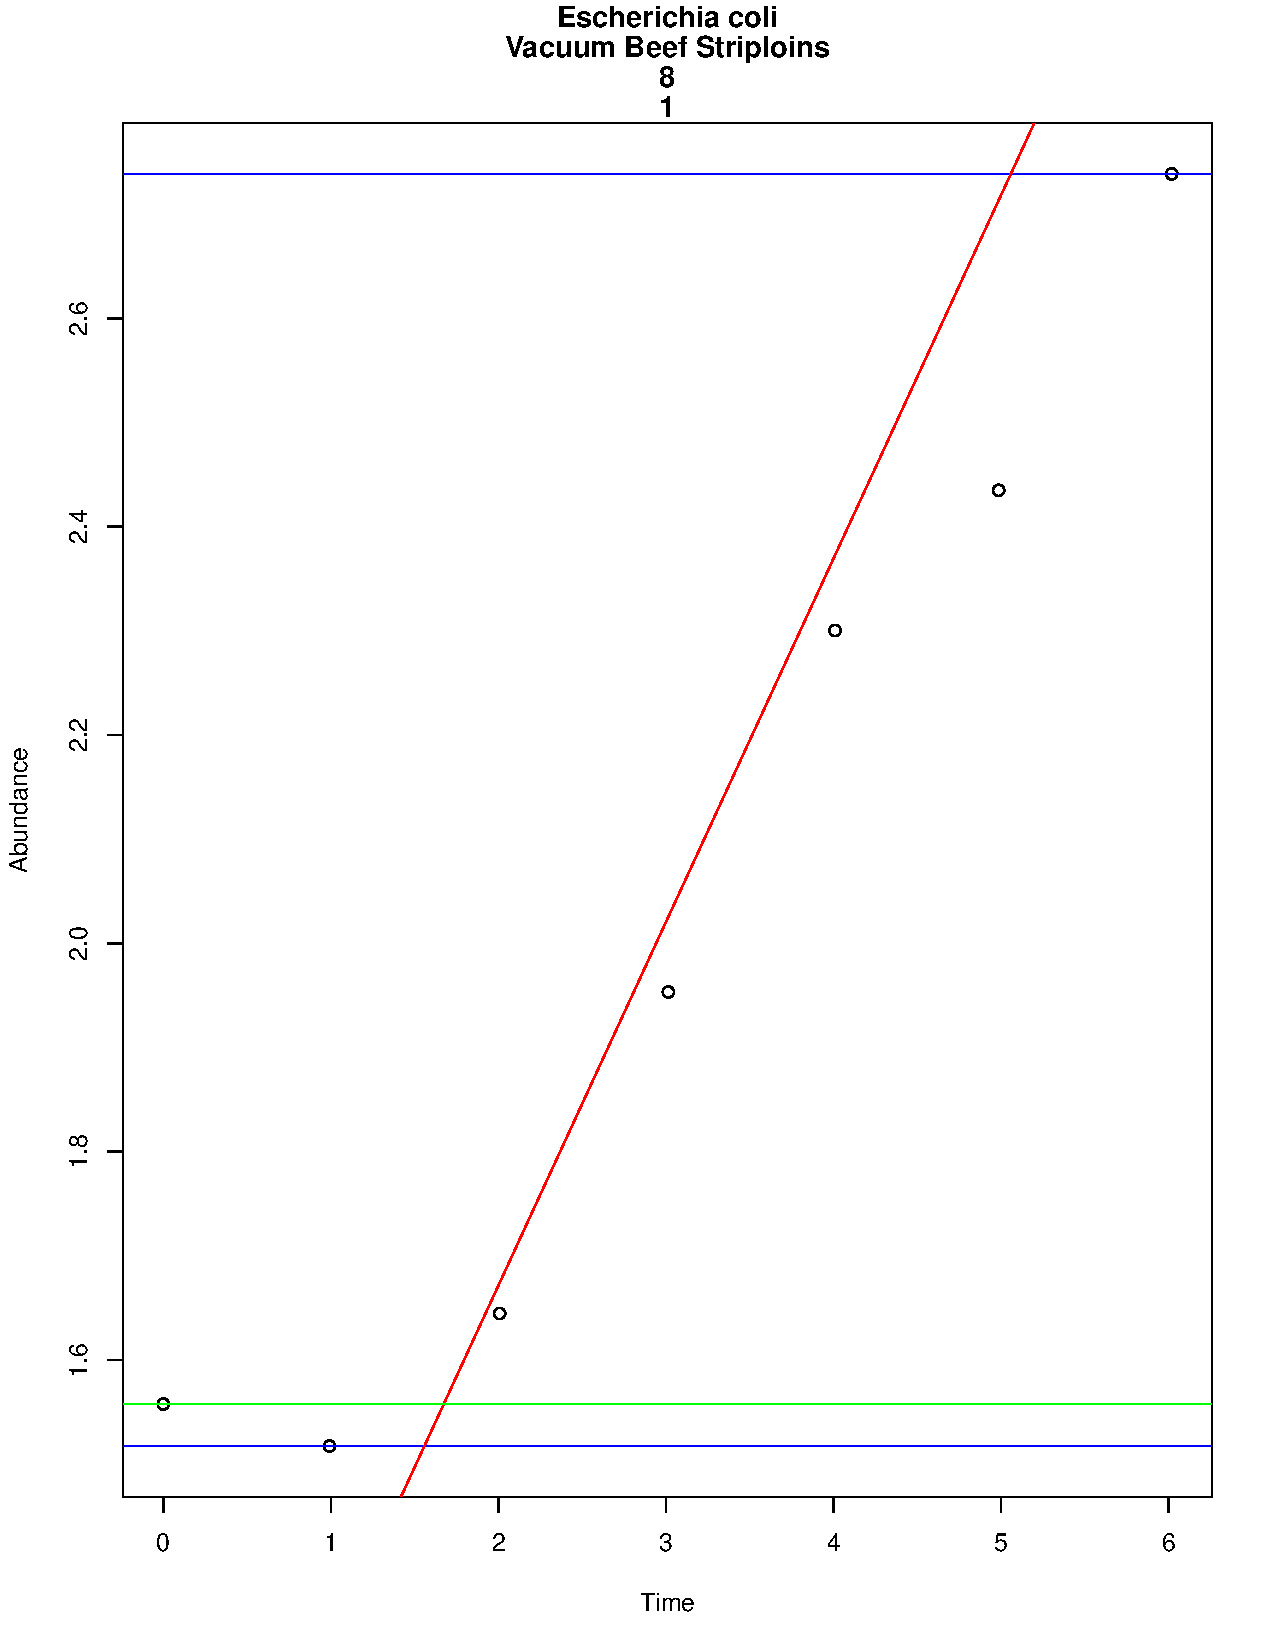
\includegraphics[scale=0.5]{../Results/Parameters_Ecoli.pdf}
\caption{The first replicate of species Escherichia coli grown in medium of Vacuum Beef Striploin at a temperature of 8\degree C. The blue lines represent $N_0$ (lower blue line) and $N_{max}$ (upper blue line). The red line represents the slope representing $r_{max}$. Finally the green line is the estimate of the $t_{lag}$, where x-value of the intersection of the red and green is the parameter estimate.}
\label{fig:Starting parameters}
\end{figure}

Species and medium were the factors accounted for when identifying the correlation between temperature and growth rate. For each of the unique ID’s, the growth rates, temperatures, Species and growth medium were recorded in a large matrix. The matrix was subset to the different unique ID’s and linear regression analysis was done to analyse the correlation.

\subsection{Fitting the models}

The R software will be used to test the models and their fits. Using the package \textit{minpack.lm}, the \textit{nlsLM()} function is used to fit the non-linear mechanistic models. Since it is non-linear regression fitting, parameter starting values must be estimated within range of the global maximum or minimum respectively as unlike linear regression, the function can find an optimal value, but only be a local minimum or maximum. To fit the Baranyi, Gompertz and Buchanan models, it requires inputting four starting parameter values ($N_0$, $t_{lag}$, $r_{max}$, $N_{max}$) for the parameters of the equation, while the Logistic model does not require a starting $t_{lag}$.

\subsection{Fitting Analysis}

All models were fitted on all of the data and the best fits were analysed using the Akaike Information Criterion (AIC), which measures the amount of lost information when fitting the models \cite{posada2004model}. We are using AIC to assess the model fit as it is able to analyse nested and non-nested model fits as well as being less penalising for additional parameters unlike BIC \cite{posada2004model}. In this case, the four mechanistic models which all have similar parameters with $t_{lag}$ being the additional parameter.

\subsection{Additional investigation}

Aside from identifying the best fit model, another aspect being investigated is the correlation between growth rate and temperature. The models used despite their derivations contain the same parameters, having a unified theory for the bacterial growth behaviour \cite{levins1966strategy}. Investigating how the growth rate changes as temperature increases through linear regression analysis. Each of the unique species and mediums will give insight if the trend is consistent. A linear regression was compared to the formula found in the paper of \textit{Ratkowsky et al.} The correlation coefficients from the linear regression and p-values of the slope coefficients were recorded and saved in a table.

\section{Results}
Filtering and wrangling the data resulted in 305 different unique sub-data sets being produced, saving the data frames of time and common logarithm of the population, and the respective unique species ID in \textit{.rda} files. The plots to show the trend in population over time has time along the x-axis and Abundance along the y-axis. Plots revealed an inconsistent distribution of the data set. Distribution were either sigmoidal, log distributed or completely random.  All starting parameter values were generated for 298 of the 305 data sets.

Optimal parameter values were obtained for most of the unique data sets. The Buchanan model had 105 fits, Baranyi model had 218 fits, Gompertz model had 211 fits and finally the Logistic model had the most with 241 fits. The models fit approximately 80% of the data. Of the 305 data sets, 243 total model fittings were successfully produced. From the 243 fittings, the best model was the one with the lowest AIC value. The distribution of best fit was uneven among the four models, as majority of the relative best fits was by the Gompertz model, with 99 of the 243, while the next best fit was the Baranyi model with 66, and Logistic and Buchanan with 51 and 27 respectively.
\begin{figure*}[h!]
    \centering
    \begin{subfigure}[h]{0.4\textwidth}
        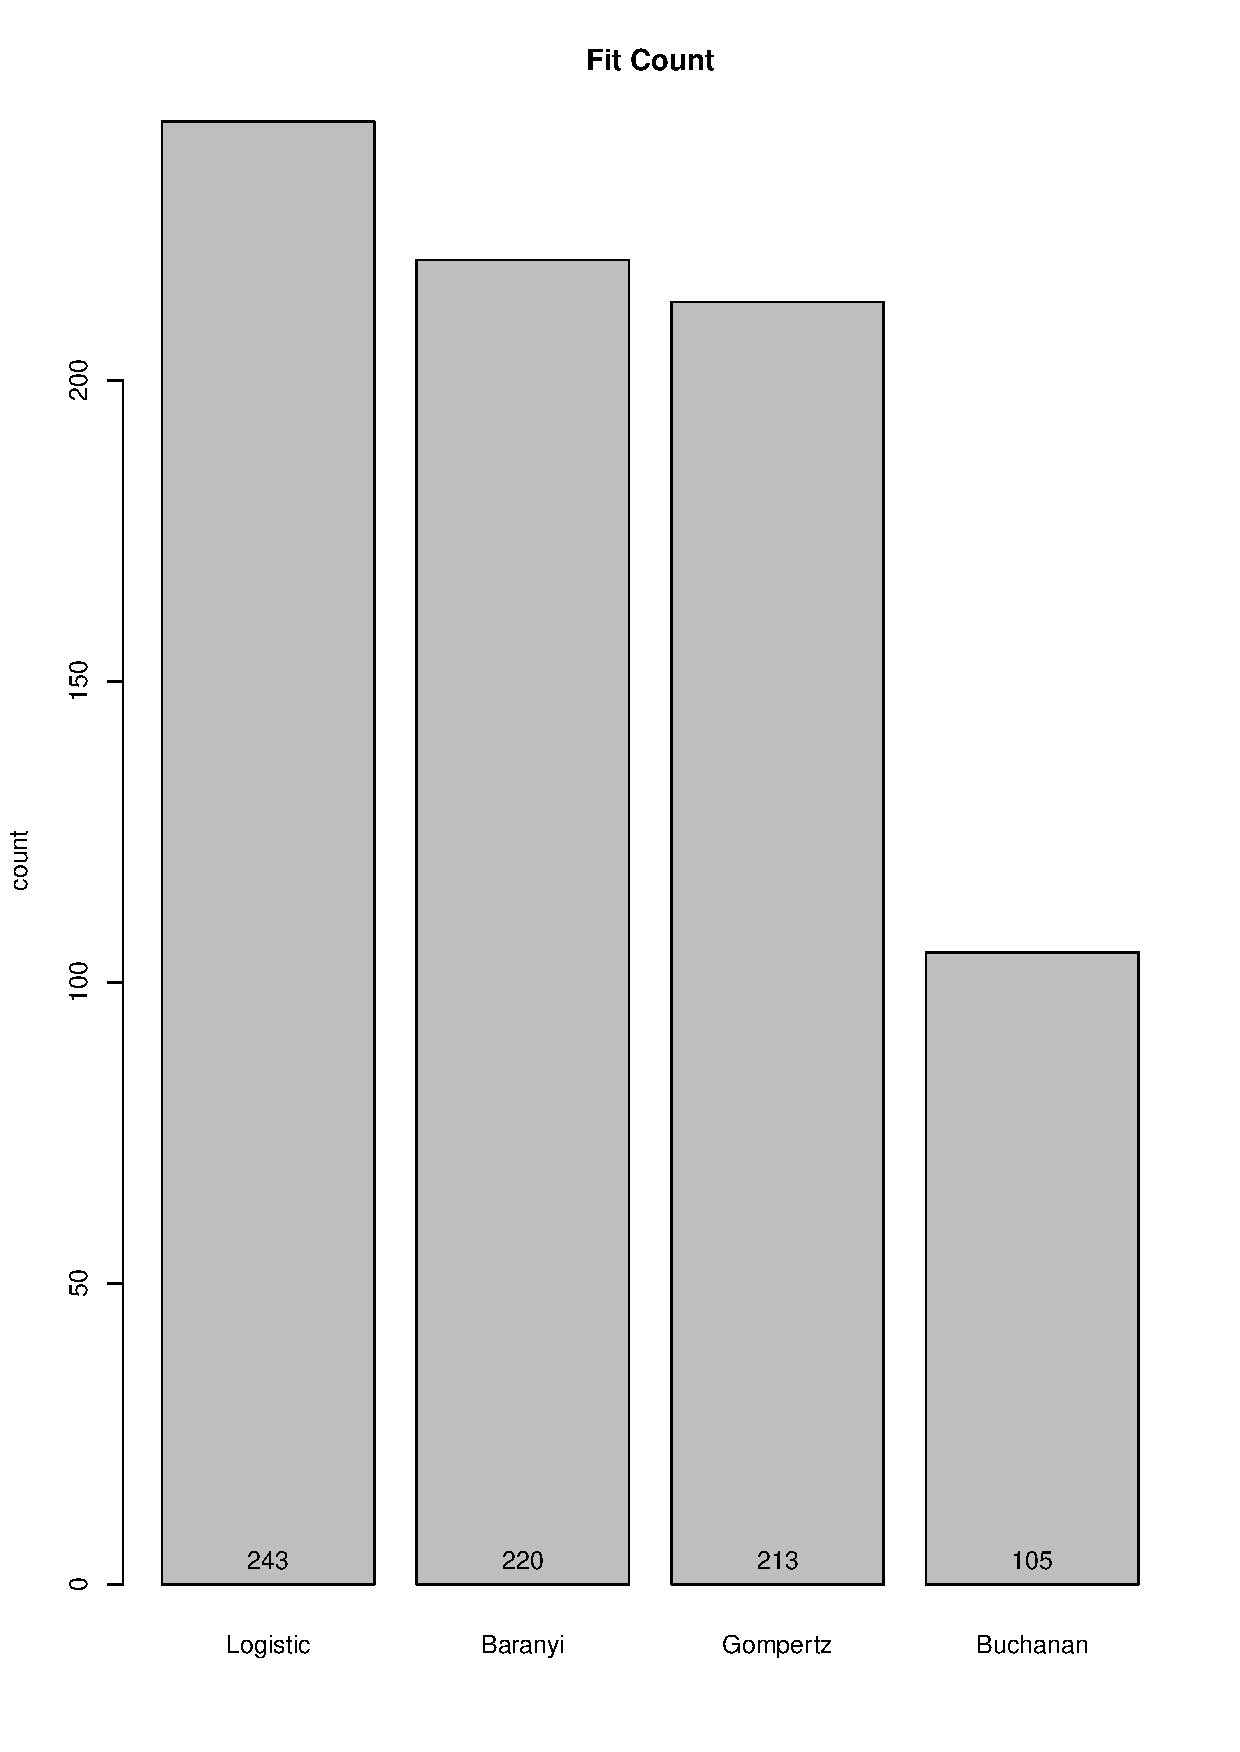
\includegraphics[width=\textwidth]{../Results/Fit_count.pdf}
        \caption{Figure 2.1: Barplot of the number of successful fits for each model}
        \label{fig:Fit Count}
    \end{subfigure}
    \hfill
    \begin{subfigure}[h]{0.4\textwidth}
        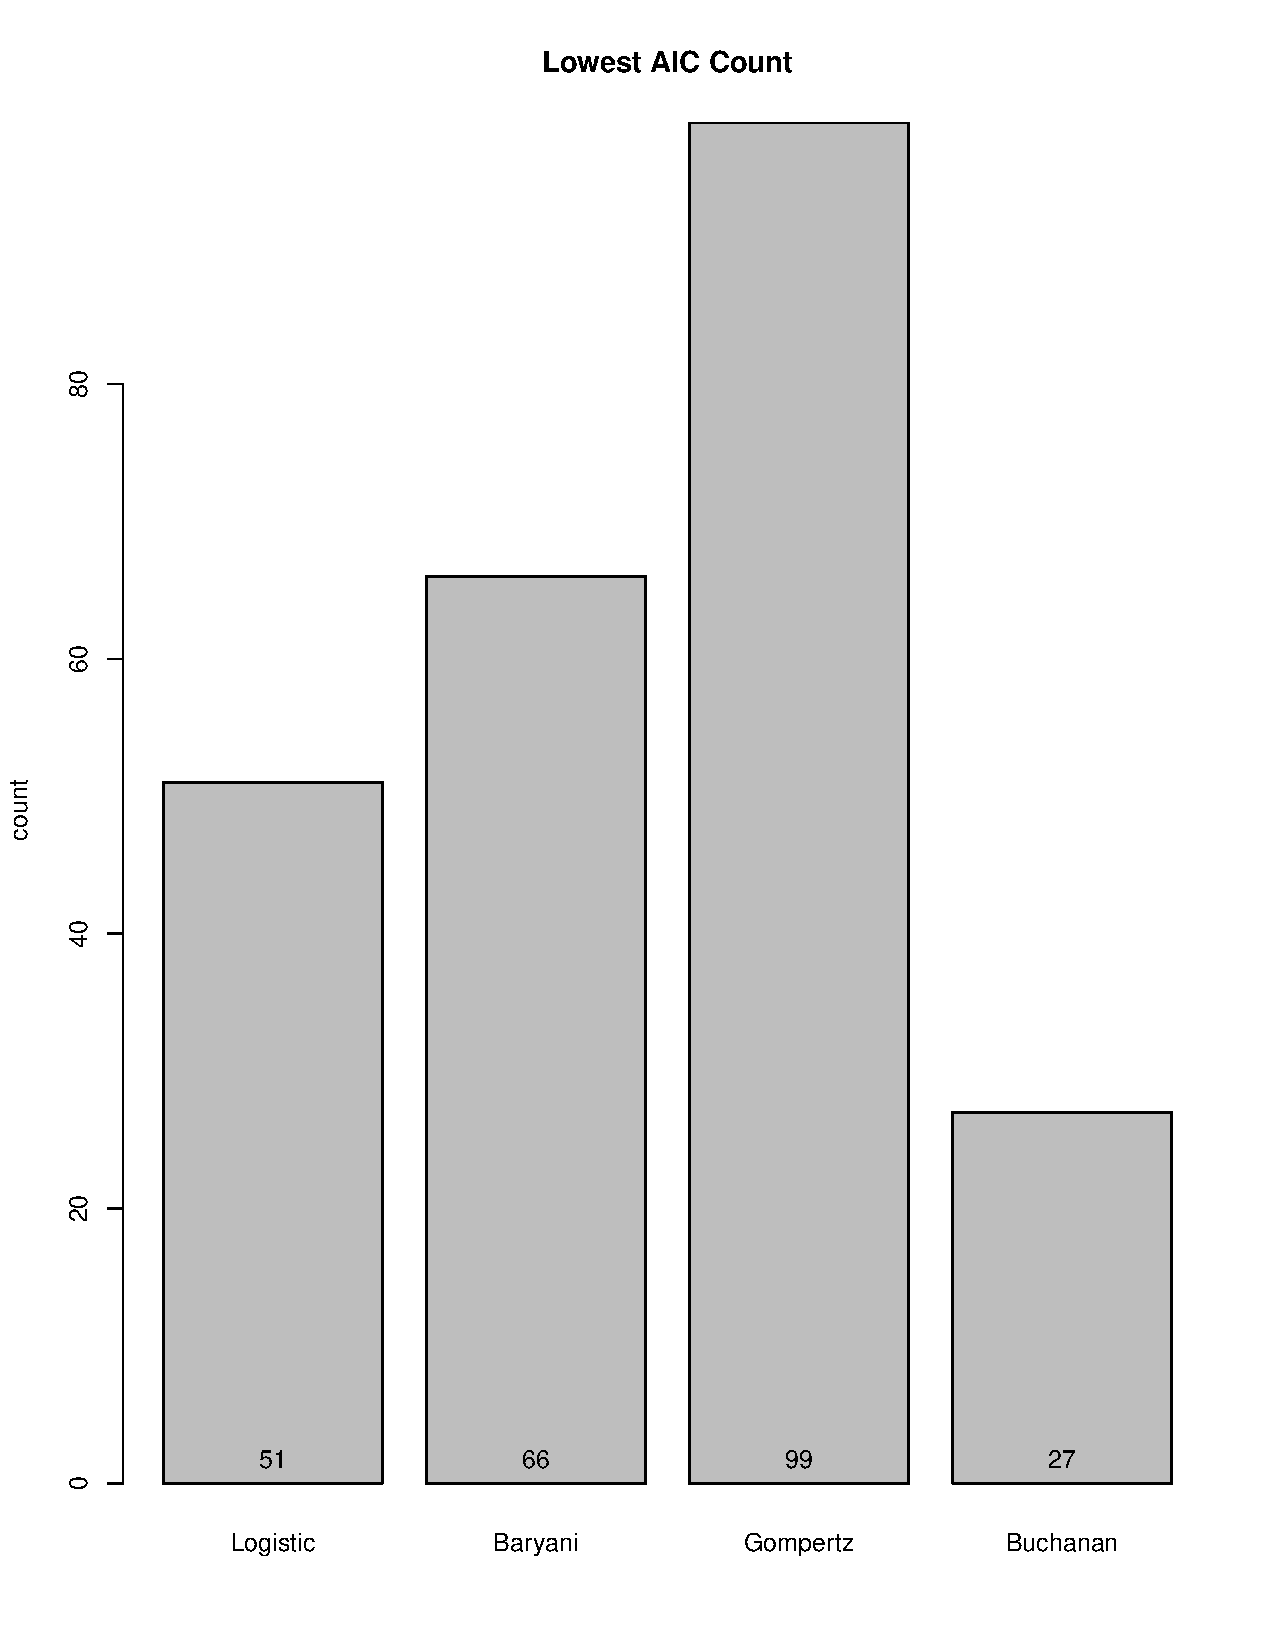
\includegraphics[scale=0.35]{../Results/bestfit_barplot.pdf}
        \caption{Figure 2.2: Barplot showing count of lowest AIC scores for each of the models tested on the data}
        \label{fig:AIC count}
    \end{subfigure}
\end{figure*}

In the additional investigation from the paper, conceptual temperature recordings existed for five of the species from the published data. These five species and their data were subsetted, and linear regression analysis was carried out. The plots include two lines, the linear regression line, and the formula \begin{equation*}\sqrt{r}=b(T-T_0)\end{equation*}\cite{ratkowsky1982relationship}. Temperature along the x-axis was plotted against $\sqrt{r}$ on the y-axis as recommended by \textit{Ratkowsky et al.} Visualisation of the results shows that the growth rate is positively correlated with temperature, with an average value of 0.958, with an overall p-value of $1.01\cdot10^-9$ for the slopes. This suggests very strong positive correlation between growth rate and temperature. Temperature is treated to be a continuous variable and as the temperature increases, growth rate will increase as well. \textit{Ratkowsky et al.} showed plotting the square root growth rate against the temperature values, allows for linear analysis, however the equation did not fit the data as well as the linear regression.
\begin{table}[h!]
\centering
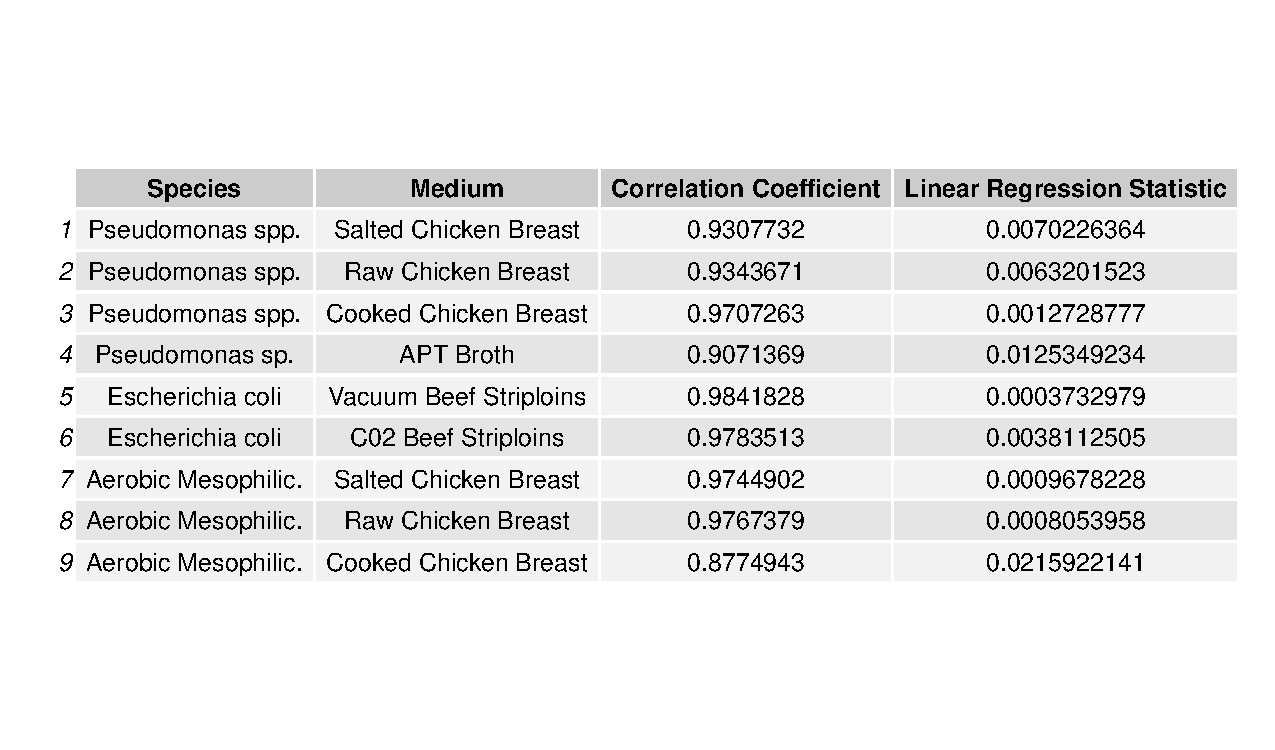
\includegraphics[scale=0.40]{../Results/Temperature_Growthrate.pdf} \caption{Correlation coefficients of square root growth rate and temperature} \label{tab:Correlation Table}
\end{table}

\section{Discussion}
\subsection{Wrangled data and starting parameters}
\begin{wrapfigure}{r}{0.4\textwidth}
    \begin{center}
        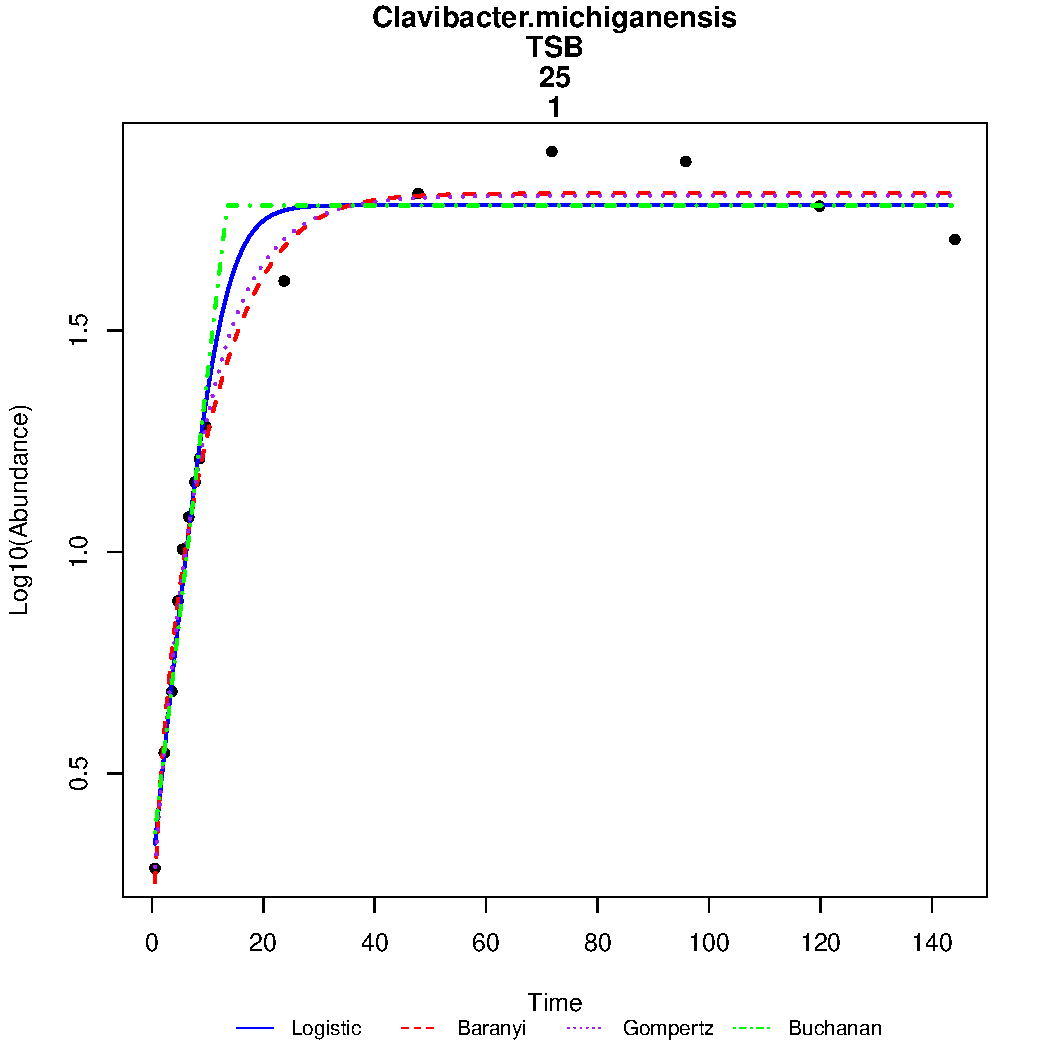
\includegraphics[width=0.48\textwidth]{../Results/Cmichiganensis25_fit.pdf}
    \end{center}
    \caption{Clavibacter michiganensis model fit showing the death phase}
    \label{fig:Clavibacter michiganensis}
\end{wrapfigure}

Distribution of the data sets were not consistent as some plots revealed no pattern, having a random distribution of points along the axis, unable to derive starting parameter values and overall fit the models. Furthermore, some of the data sets revealed a decline once the asymptotic value has been reached. This is the death phase which is ignored in the model fitting process \cite{zwietering1990modeling}. Getting all required starting parameters was necessary for the model fittings to be produced. Despite not all the data sets having a sigmoidal or log distribution, positive $r_{max}$ and  $t_{lag}$ values were still derived from all the data sets. Although the Logistic model only requires three of the starting parameters, the growth rate parameter is the determining factor of all the models fitting. Starting population ($N_0$) and carrying capacity ($N_{max}$) are easily derived from the data sets however, growth rate and time lag are mathematical derivations, thus have the possibility of having NA values depending on the distribution of data points. The growth rate coefficient represents the max slope between points, which is the derivative along the inflection point. While the $t_{lag}$ requires the y-intercept of $r_{max}$ slope as well as the actual slope value to derive it.

\subsection{Model fitting}
\begin{figure*}[h!]
    \centering
    \begin{subfigure}[h]{0.4\textwidth}
        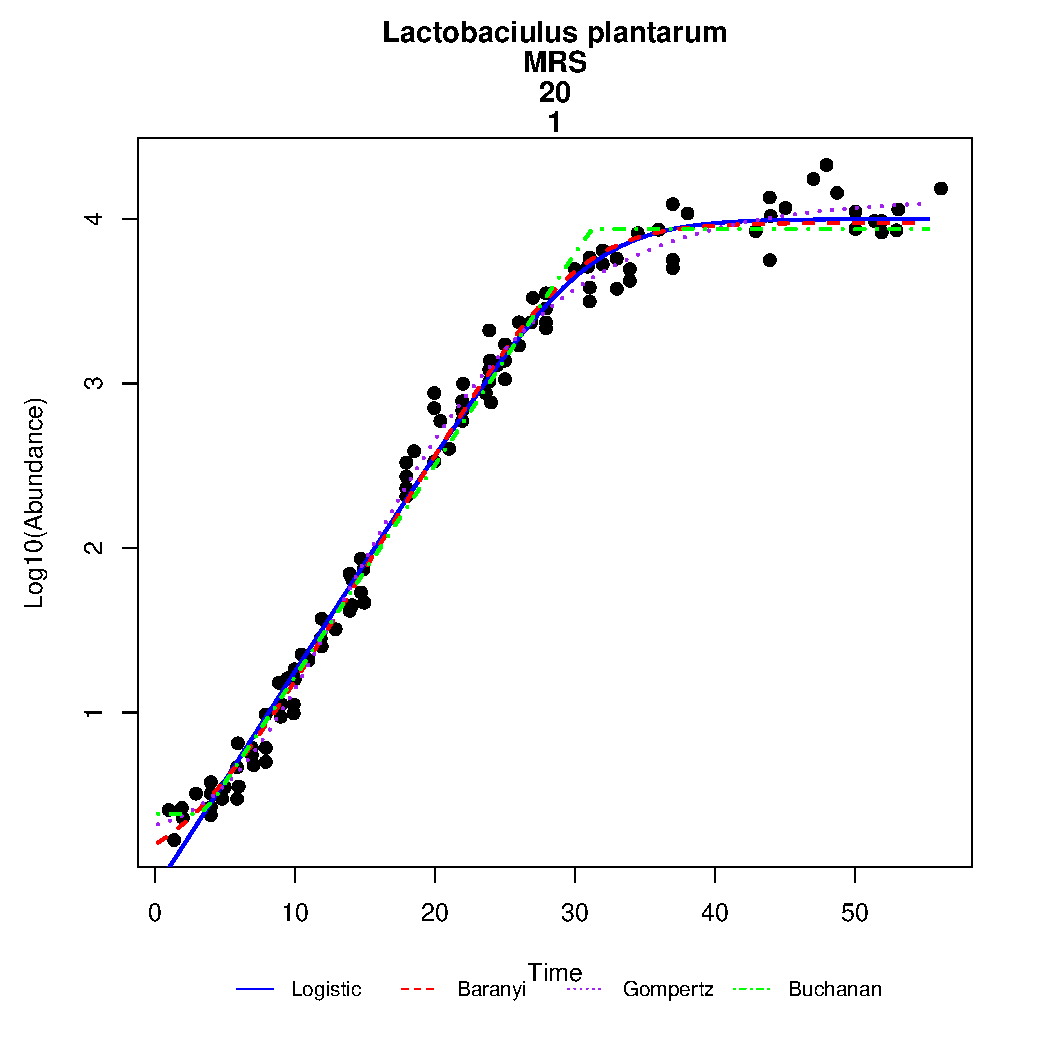
\includegraphics[width=\textwidth]{../Results/Lplantarum_fit.pdf}
        \caption{Figure 3.1: Lactobaciulus plantarum model fit}
        \label{fig:Lactobaciulus plantarum}
    \end{subfigure}
    \hfill
    \begin{subfigure}[h]{0.4\textwidth}
        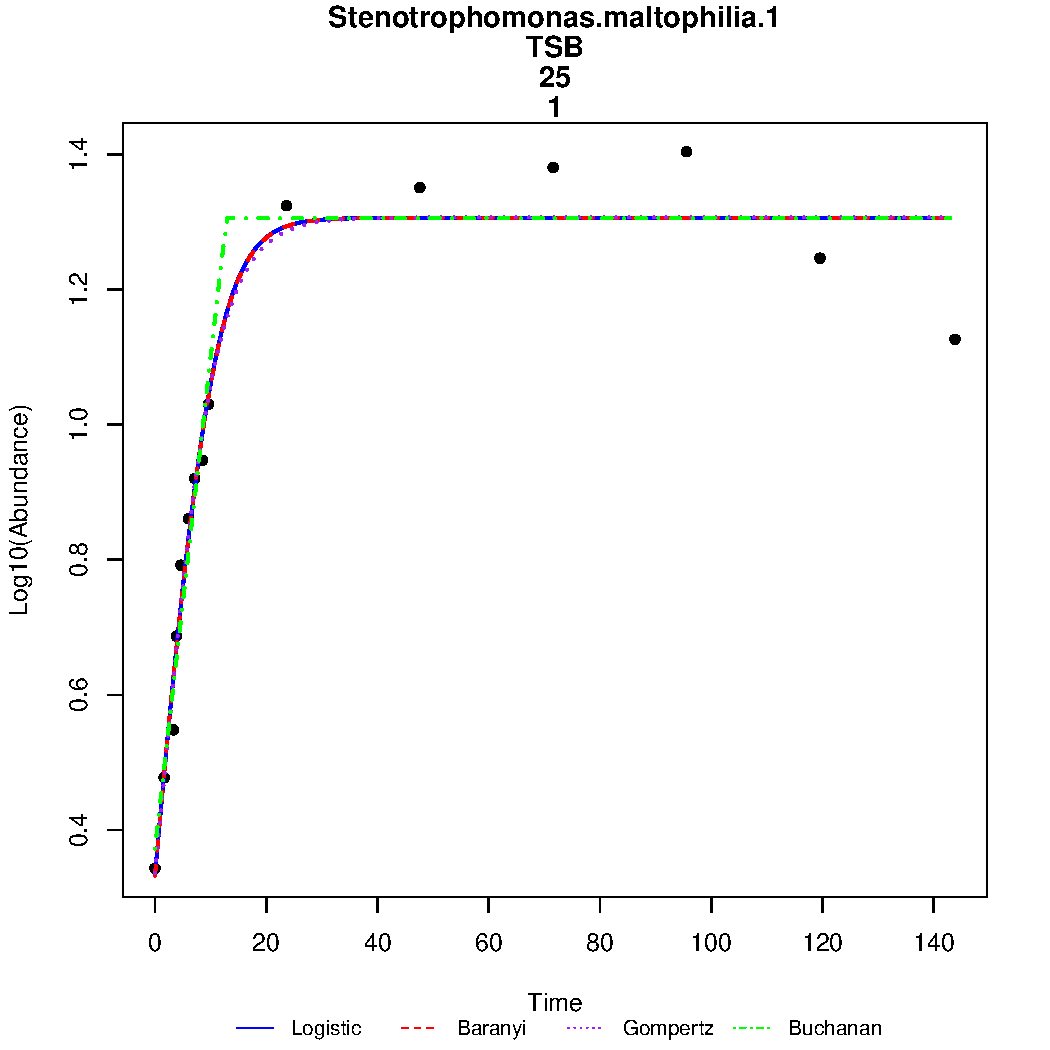
\includegraphics[width=\textwidth]{../Results/Smaltophilia25_fit.pdf}
        \caption{Figure 3.2: Stenotrophomonas maltophilia model fit}
        \label{fig:Stenotrophomonas maltophilia}
    \end{subfigure}
\end{figure*}

All four models were nested upon each other, utilising similar parameters. The Logistic model is derived from external limiting factors including resource and density. These external factors play limit the exponential growth of the population, hence producing the sigmoidal shape where it reaches an asymptotic value \cite{webb1986logistic}. The Baranyi model is a differential model which accounts biological factors of individual microbial growth. It takes into account environmental variation and the physiological limiting factors, specifically the limits in the rate of biochemical reactions within the microbe \cite{buchanan1997simple, grijspeerdt1999estimating}. The Buchanan model is a simplified version of the Gompertz model and Baranyi model, which accounts for biological variability, considering individual physiological factors and population factors such as adaptation at each of the growth phases to produce a three-phase linear model \cite{buchanan1997simple}.

Overall, the results show that the Gompertz model was the most robust model, having the greatest number of goodness of fit. In other words, for the provided data set, it is the best model to describe the population dynamics of microbial growth over time. This is not surprising as it is a primary level model, which only describes change population over time \cite{grijspeerdt1999estimating}. The Gompertz model is mathematical derivations to form the sigmoidal relationship \cite{buchanan1997simple} et al., 1997). Despite its parameters, it is an empirical derivation not accounting for any biological processes. The robustness of the model is from the parameters. The parameters account for shape or curvature of the fit, and location along the axis, allowing the model to shift the fit along the x-axis or y-axis and maintain its overall shape \cite{tjorve2017use}. Furthermore, similar to the method of deriving the growth rate from the data sets, the growth rate in the Gompertz model is derived along the inflection point.

\subsection{AIC}

Best fitting model was determined through the AIC values produced. From the results, the Gompertz model was the most robust, having the most number of fits. This is due to the derivation and robustness of the parameters, as well as the flexibility of the model \cite{tjorve2017use}. Depending on the data set, the AIC values produced negative or positive ranges of values, and the best model fit was the model that produced the minimum value relative to the other fits. The AIC values here shows that Gompertz model most likely explains the data sets however, cannot explain how “true” realism, since we are only comparing relatively between the four models. AIC considers the trade-off between model complexity and fit \cite{vrieze2012model}. AIC does favour more complex models as from the formula, the $-2 \cdot \mathcal{L}$ is decreased, which is why the Gompertz model performed well as it contains four parameters \cite{posada2004model}. The extra parameter in addition with the flexibility of the model itself makes it a robust fit.

\subsection{Temperature and Growth Rate Correlation}
\begin{table}[h!]
\centering
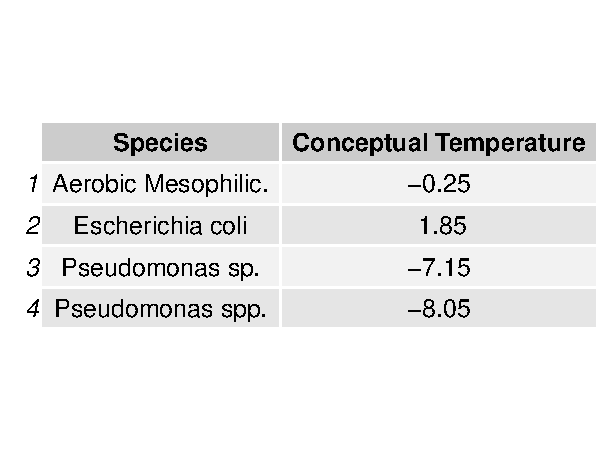
\includegraphics[scale=0.60]{../Results/Species_ConceptualTemp.pdf} \caption{Provided conceptual temperatures of species in data set} \label{tab:Conceptual Temperature}
\end{table}

Using the species with recordings of conceptual temperature, the plots show that there is a strong positive correlation between growth rate and temperature. A linear regression analysis was done and also fitting the the formula given from \textit{Ratkowsky et al.} Unlike the original paper, the distribution of points were not as linear but this is likely due to data collection methods from the data provided as well as physiological differences of the species. Using the linear regression analysis, x-intercept values were calculated to see if they coincide with conceptual temperatures \cite{ratkowsky1982relationship}. The x-intercepts vary from the conceptual temperatures provided from the paper. From the plot, aside from the \textit{Aerobic Mesophilic} in \textit{Cooked Chicken Breast}, the Conceptual Temperature model did not align with the data well.

\begin{wrapfigure}{r}{0.3\textwidth}
    \begin{center}
        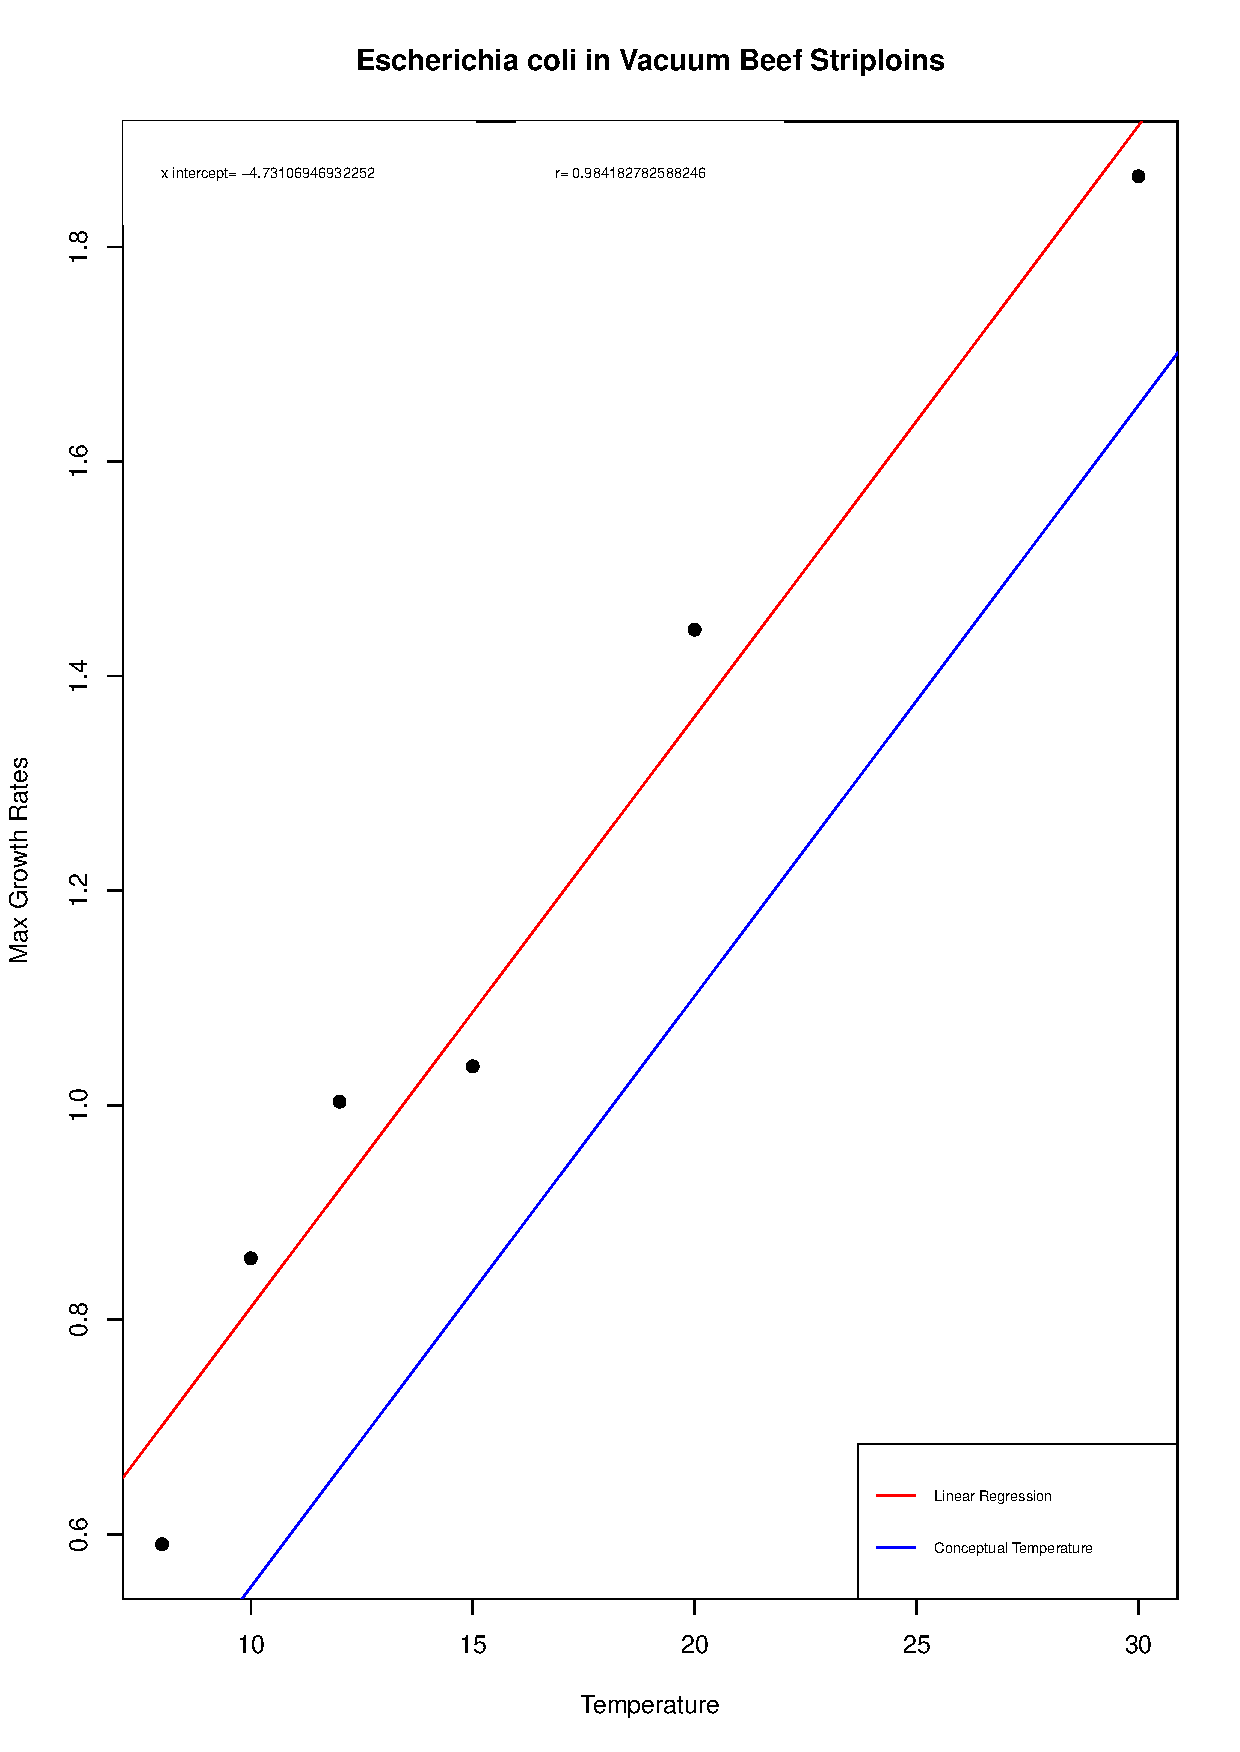
\includegraphics[width=0.40\textwidth]{../Results/Ecoli_r_temp.pdf}
    \end{center}
    \caption{Escherichia Coli recorded growth rates plotted against temperature}
    \label{fig:E.coli correlation}
\end{wrapfigure}

Furthermore looking at the regression analysis, if we use a significance value of 0.05, using fisher’s method for independent test statistics, which takes the logarithm of the p-values \cite[p.103]{fisher1992statistical}. The resulting p-value is much less than the significant level. This means that the slopes are statistically significant, not random and support the positive correlation between temperature and growth rate. Only five species were investigated but further analysis can be done as conceptual temperature values are collected for the other species in the provided data. Overall, the results show that temperature and growth rate are positively correlated.\\

\section{Conclusion}
In conclusion, the Gompertz model performed well due to its derivations. As mentioned in the Discussion, the parameters and its values are empirically derived. Similar to the Logistic model, its parameters do not consider the physiology or limiting factors of the organism, just the rate at which it divides. Furthermore, compared to the Logistic model, it takes in an extra parameters that makes it more robust and flexible.

When fitting models, there is a tradeoff between realism and complexity. Although complex models, which contain more parameters, it will fit the given data set better. This is however, all dependent on the context and purpose of study. In this research, the focus was on  models that can explain the patterns and trends in this data set, and would fit well relative to the others. In reality, models should consider other data sets as well, being able to consistently describe the trends. Furthermore, take into account biological processes to have proper meaning. Only two models, Baranyi model and Buchanan model actually considered organismal physiology and further model fitting can be done using other biologically mechanistic models that take into account internal and external factors.

For the additional investigation, although the distribution of the data did not match that from the study carried out by \textit{Ratkowsky et al.}, and only used five species, the overall result still supports that growth rate is positively correlated to increases in temperature. The derived conceptual temperature from the linear regression did not match that provided from the paper but that is likely due to lack of replications.

\newpage

\section{Data Code and Availability}
All code can be found in the GitHub Repository:\\
{https://github.com/matthewcampos/CMEECourseWork.git}

\newpage

\bibliographystyle{agsm}
\bibliography{references}

\end{document}
